\documentclass{report}
\usepackage{geometry}
\geometry{ a4paper,total={170mm,257mm}, left=20mm, top=20mm}
\usepackage{sagetex}
\usepackage{fancyhdr}
\usepackage{amsmath}
\usepackage{subcaption}
\usepackage{enumerate}
\usepackage{pgfplotstable}
\usepackage{booktabs}
\newcommand{\code}[3][IS]{#2:#3}
\newcommand{\figmacro}[1] {Fig. #1}
\newcommand{\equmacro}[1] {Equation #1}
\newcommand{\chartmacro}[1] {Chart #1}
\newcommand{\tablemacro}[1] {Table #1}
\newcommand{\Fefouronefivemacro}[1] {$Fe$ 415 #1}
\newcommand{\Fefivezerozeromacro}[1] {$Fe$ 500 #1}
\newcommand{\Fetwofivezeromacro}[1] {$Fe$ 250 #1}
\DeclareCaptionType[fileext=loc]{chart}[Chart][List of Charts]
\usepackage{graphicx}
\usepackage[autostyle]{csquotes}
\usepackage[backend=biber]{biblatex}
\addbibresource{chapter12.bib}
\title{Individual Spread Footing}
\author{Manpreet Kaur, Amritpal Singh}

\begin{document}
\maketitle
\tableofcontents
\listoffigures
\listofcharts
\listoftables
\setcounter{chapter}{11}
%----------------------main document start------------------%
\chapter{Individual Spread Footing}
\section{Introduction} Clause 34 of the  \citetitle{IS2000} gives the provisions
governing the design of reinforced concrete footings.  These provisions are
similar to those given by the ACI Code. The design of footings in
accordance with \citetitle{IS2000} differs from that by
the \citetitle{IS1964} in the following aspects.

\begin{enumerate}[I]
\item Perimeter shear stress must not exceed the allowable value. This
aspect was not given in the \citetitle{IS1964}. But it is similar to the familiar
concept of punching shear stress.

\item Bond-stress-criterion was given in the \citetitle{IS1964}, but it is omitted in
the \citetitle{IS2000}. Instead, development length of footing bars is required to be
checked at the sections where bending moment is critical.

\item 25\% excess pressure on edge of footing was allowed by the \citetitle{IS1964}
when a footing is eccentrically loaded. This concession is withdrawn by
the \citetitle{IS2000}, thereby adding to the cost of eccentrically loaded footings.
\end{enumerate}
The Code requires footings to be designed for the following limit states.

\begin{enumerate}[(a)]
\item Perimeter shear
\item Bending moment
\item Beam shear
\item Development length of footing bars
\item Development length of column bars
\end{enumerate}

\section{Types of Individual Footings} Individual spread footings can be either square or rectangular in plan, the area of a rectangular footing with sides $A$ and $B$ being given by,

\begin{equation}
\label{eq:footingArea}
A \times B = \frac{P}{p}
\end{equation}
where $P$ is the column load in $kN$ and $p$ denotes the net allowable soil
pressure in $kN/m^2$. In this development, self-weight of footing may not
be considered. This involves only a small error in that, the weight of the
concrete of footing is assumed here to be approximately equal to the weight
of the earth displaced by it. Further, it is assumed here that the soil
pressure under the footing is uniform. This is a reasonable assumption as
discussed elsewhere. Various types of  individual spread footings are shown in \figmacro \ref{Types-of-individual-spread-footing}.
%---------------figures--------------------------%
\begin{figure}
\begin{subfigure}[b]{0.5\textwidth}
  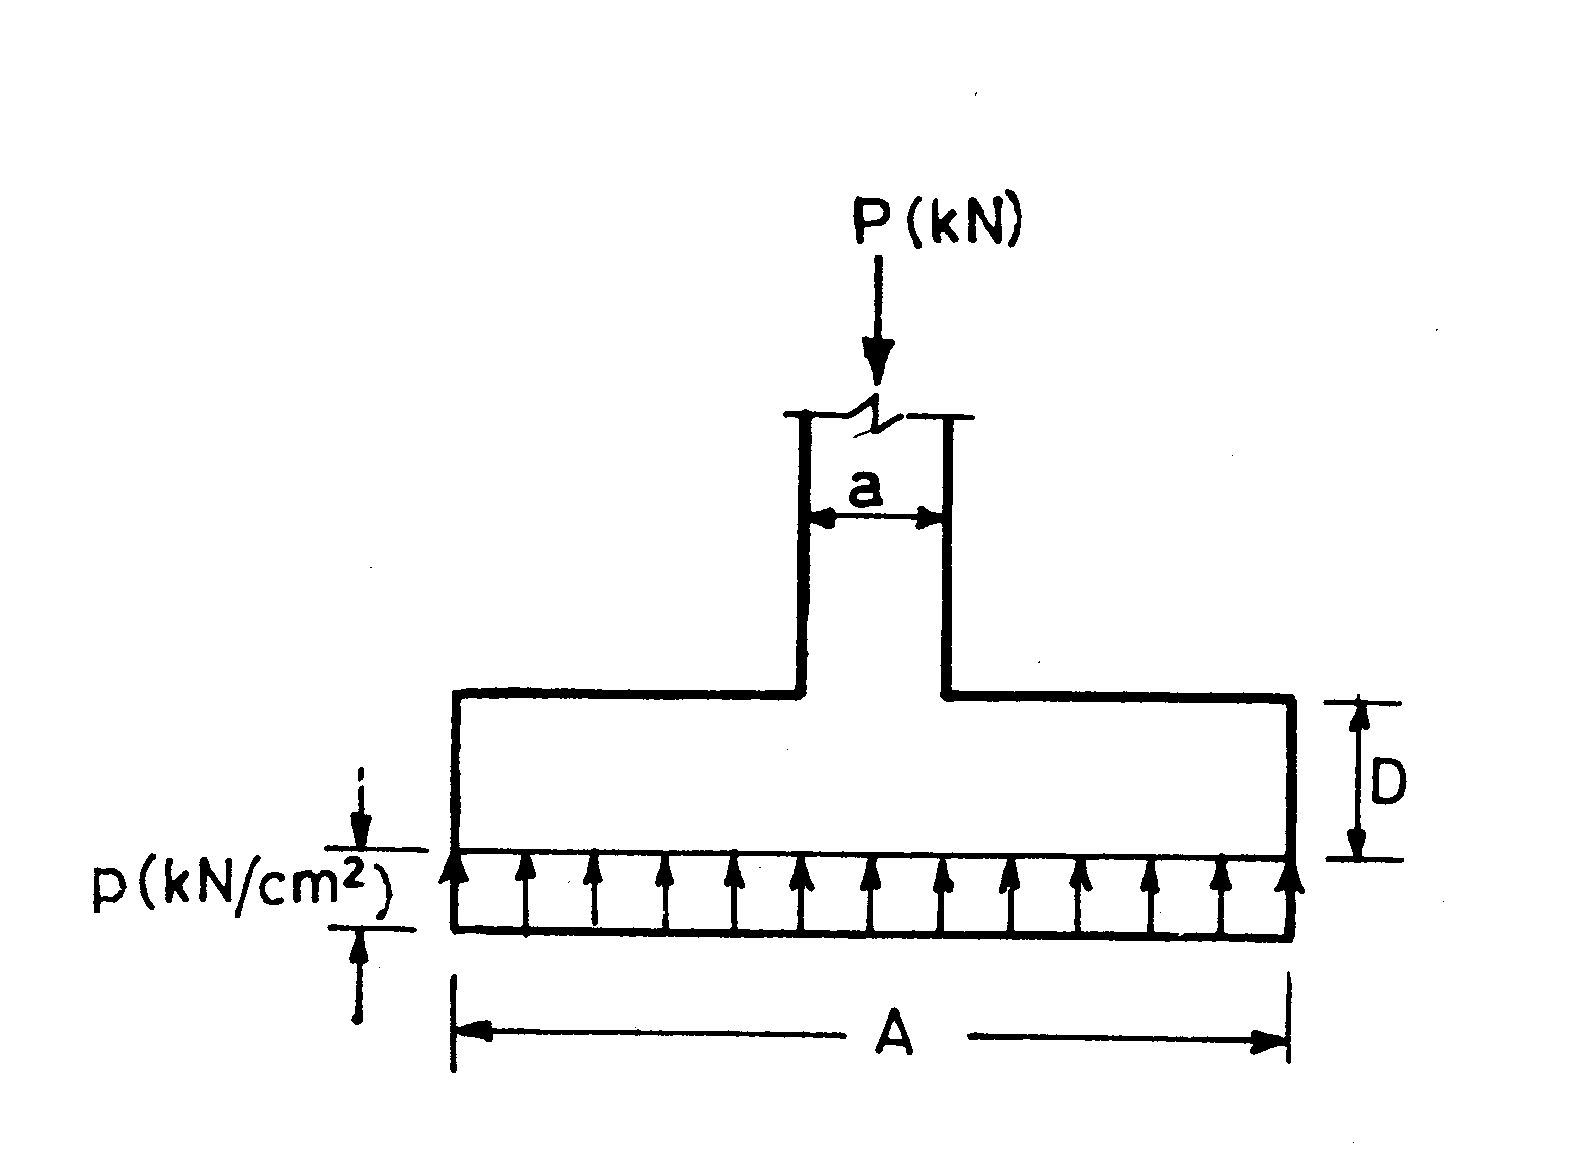
\includegraphics[width=\textwidth]{images/fig2291.png}
    \caption{Uniformly deep footing}
    \label{uniformdeepfooting}
  \end{subfigure}
  %
  \begin{subfigure}[b]{0.5\textwidth}
    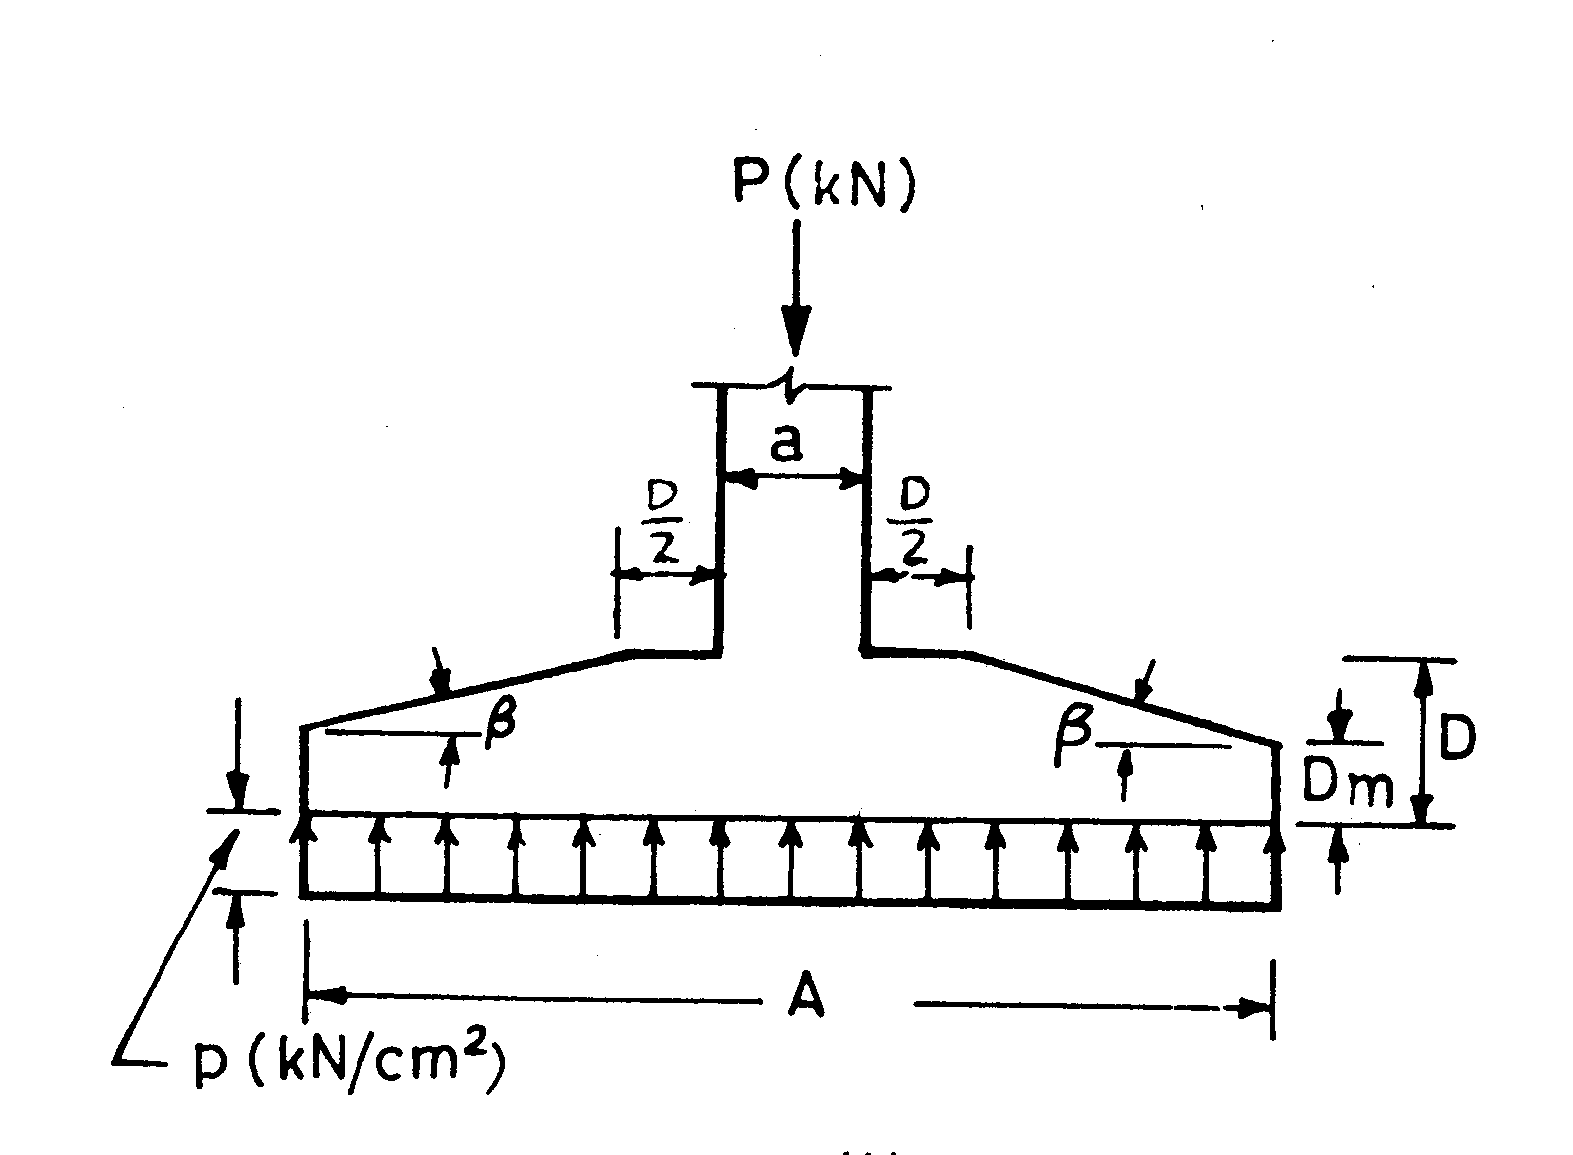
\includegraphics[width=\textwidth]{images/fig2292.png}
    \caption{Sloped footing (slope starting from $D/2$ away from the edge of column)}
    \label{Slopedfooting}
  \end{subfigure}
 %
 \begin{subfigure}[b]{0.5\textwidth}
    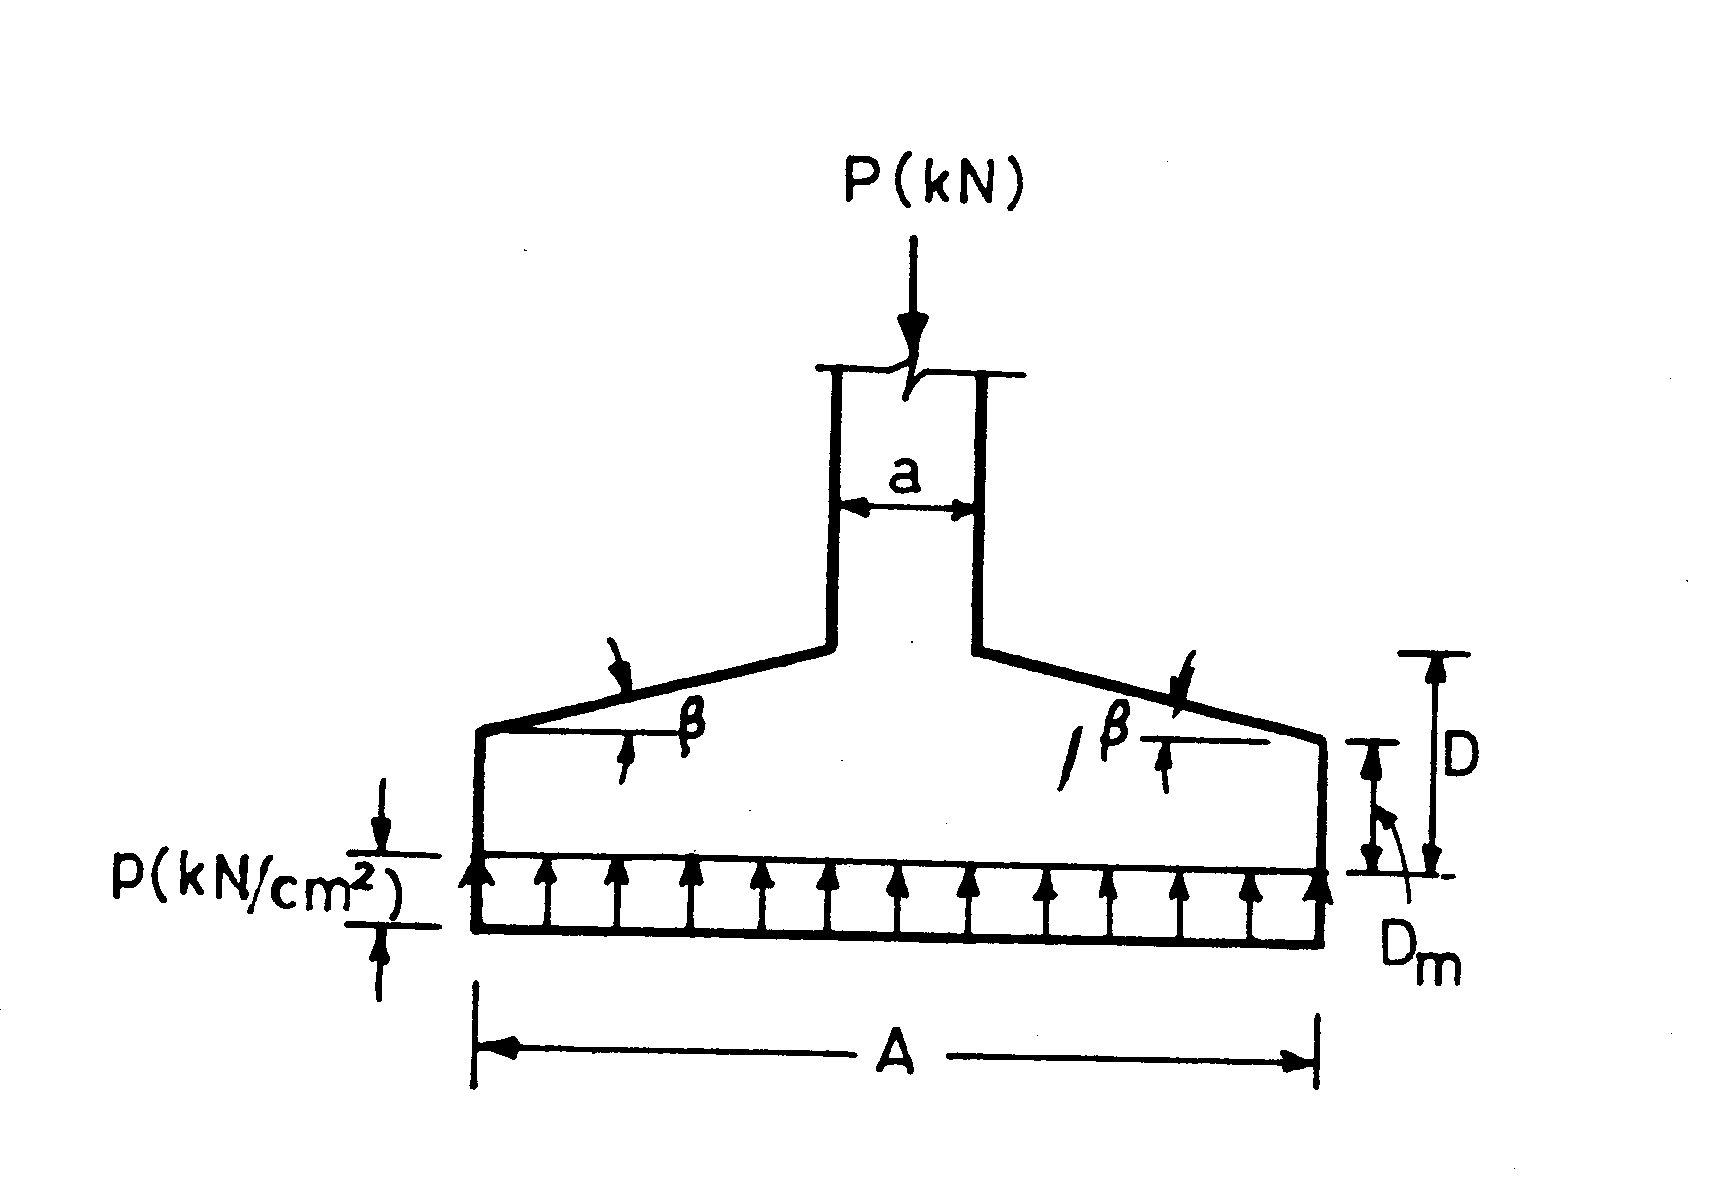
\includegraphics[width=\textwidth]{images/fig2293.png}
    \caption{Sloped footing (slope starting from the edge of column)}
    \label{slopefooting}
  \end{subfigure}
 %
\begin{subfigure}[b]{0.5\textwidth}
    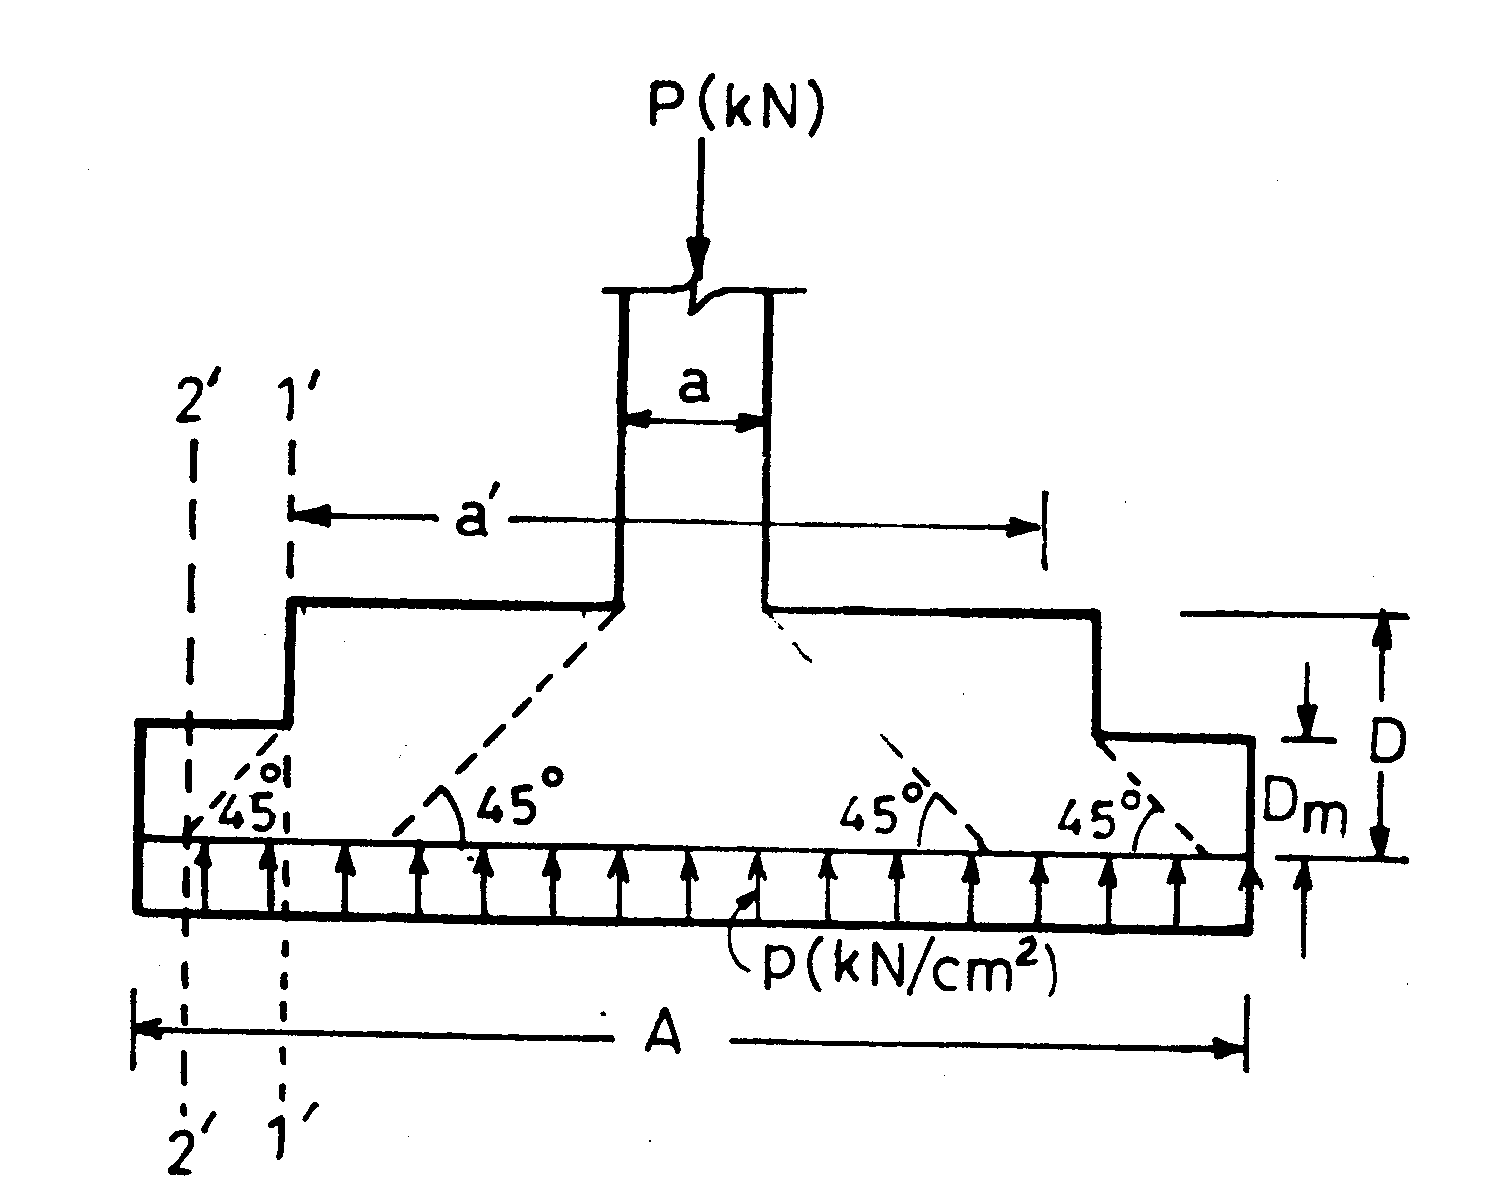
\includegraphics[width=\textwidth]{images/fig2294.png}
    \caption{Stepped footing}
    \label{steppedfooting}
  \end{subfigure}
\caption{Types of individual spread footing.}
\label{Types-of-individual-spread-footing}
\end{figure}
%-----------------end figure-----------------------%
With the area of footing known from \equmacro \ref{eq:footingArea},
dimensions $A$ and $B$ are easily finalise.  The only dimension of footing
which remains to be known is the depth ($D$) of the footing.  A common way
of design of footing is to assume D, rather generously, with a view to
reduce steel area as well as to help provide fixity to the column base, in
order to be close to the assumptions made in the frame analysis of
superstructure.

\section{Design for Perimeter Shear} Depth of footing is fixed from the
consideration of perimeter shear stress which depends on concrete quality,
being independent of types of reinforce steel. For a square footing of
uniform depth with a square column of side $a$ (\figmacro \ref{critical perimeter 1-1-1-1}), perimeter shear stress
$\tau_{v}$ is given by

\begin{equation}
\label{eq:perimeterShearStress}
\tau_{v} = \frac{V_{u}} {{b_{0}} \times d} 
=\frac{1.5 \times S_{p}} {4(a + d) \times d} 
\end{equation}
where 
\begin{equation}
\label{eq:perimeterShearForce}
\quad S_{p} = P - p \times (a + d)^2
\end{equation}
and $b_0$ = Perimeter of critical closed section.

The allowable perimeter shear stress ${\tau_{a}}$ (clause 31.6.3 of
the code) is given by,

%------------------figures---------------------%

\begin{figure}
  \centering
  \begin{subfigure}[b]{0.5\textwidth}
    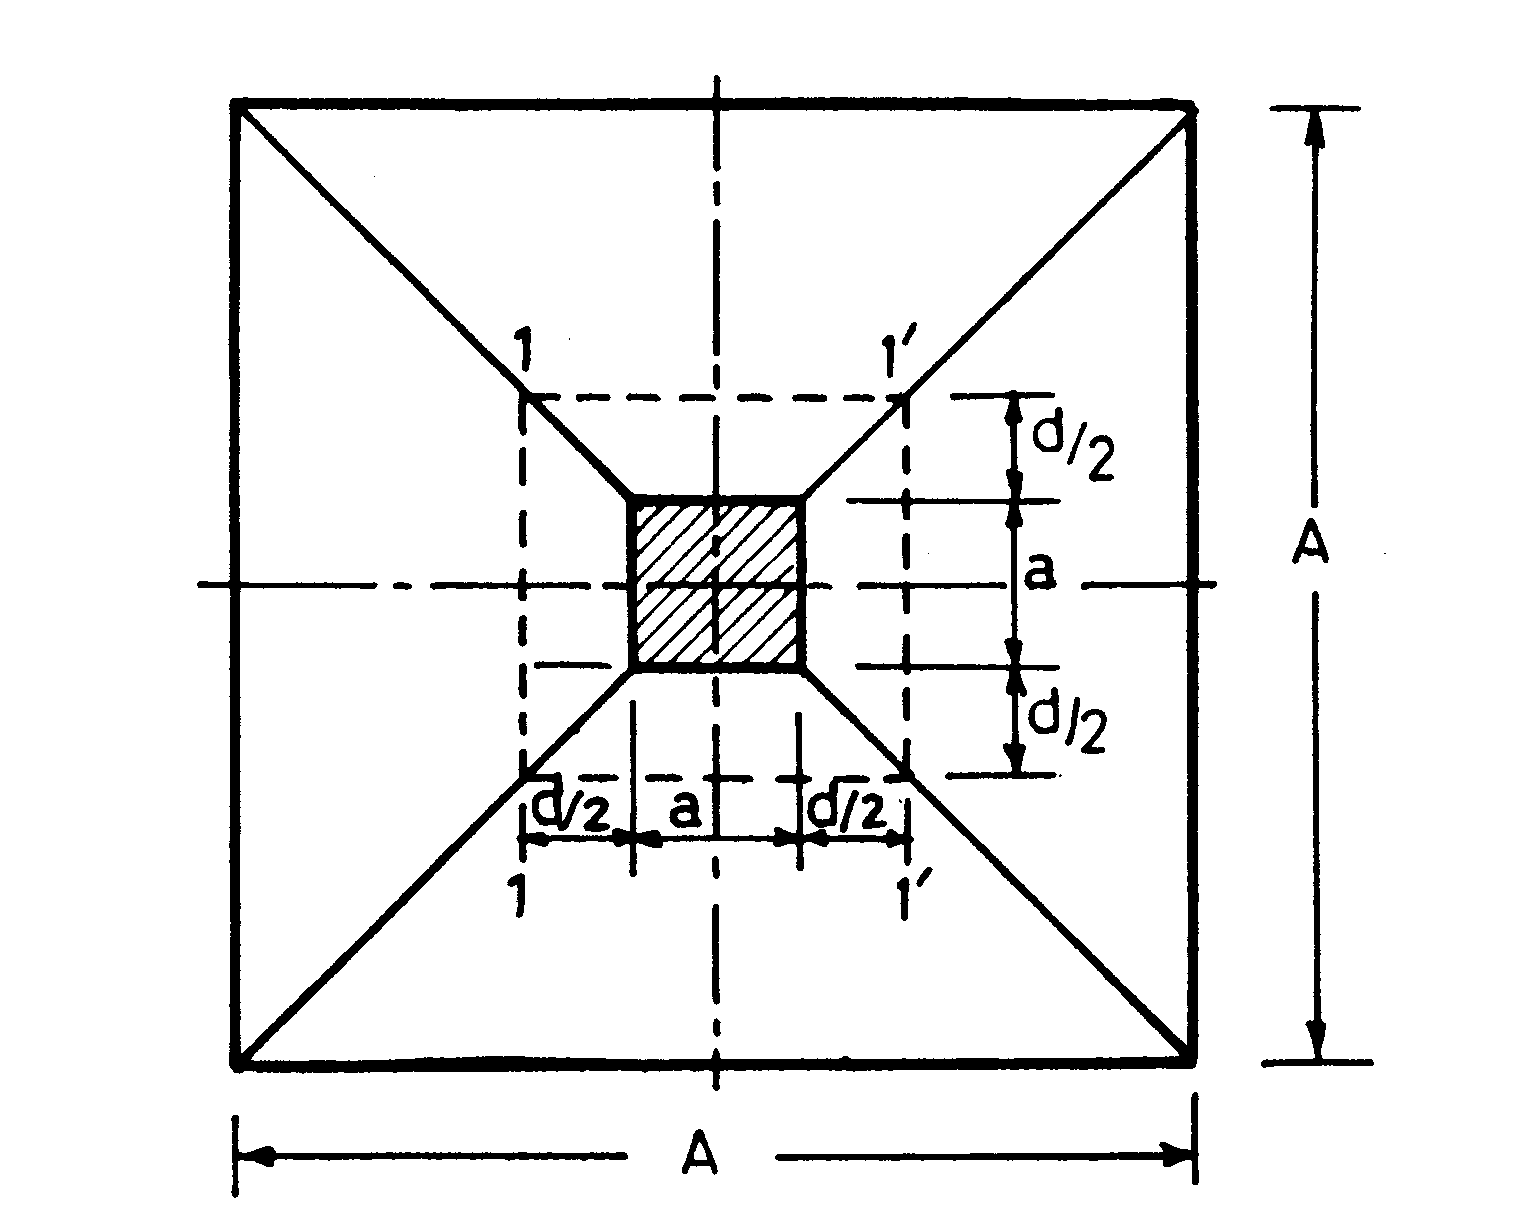
\includegraphics[width=\textwidth]{images/fig2301.png}
    \caption{Critical perimeter 1-1-1-1 in plan for perimeter shear}
    \label{critical perimeter 1-1-1-1}
  \end{subfigure}\\
  %
  \begin{subfigure}[b]{0.5\textwidth}
    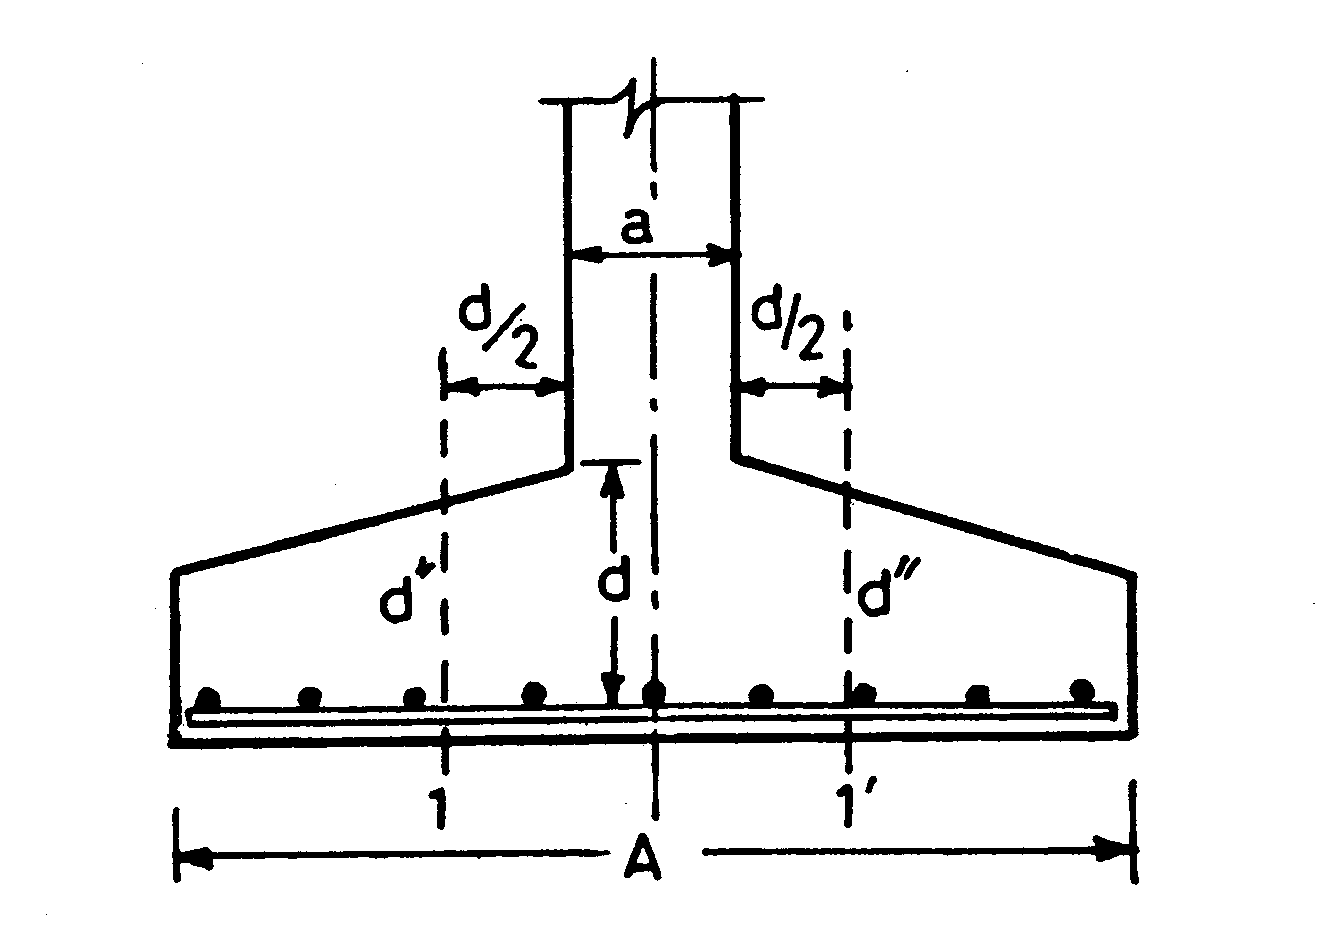
\includegraphics[width=\textwidth]{images/fig2302.png}
    \caption{Section of sloped footing showing reduced depth ${d'}$ for perimeter shear}
    \label{sectionslopefooting}
  \end{subfigure}
\caption{Perimeter shear for square footing.}
\label{Perimeter-shear-for-square-footing}
\end{figure}

%------------------end figure---------------%

\begin{equation}
\label{eq:allowable2DShearStress}
\tau_{a} = k_{s} . \tau_{c} = k_{s} \times 0.25 \sqrt{f_{ck}}
\end{equation}
where, $f_{ck}$ is to be put in $N/mm^2$.

$k_{s}$ = 1.0 for square columns and also for rectangular with aspect ratio
$\left( \dfrac{b}{a} \right) \leq {2.0}$. For the condition $\tau_{v} =
\tau_{a}$, \equmacro (\ref{eq:perimeterShearStress}) and
(\ref{eq:allowable2DShearStress}) give,

\begin{sagesilent}
  var('a,A,d,fck,p,k')
  z1=(1-(a/A)**2-2*(a/A)*(d/A)-(d/A)**2)/((a/A)*(d/A)+(d/A)**2)
  z2=(.067*fck**(1/2))/p
\end{sagesilent}

\begin{equation}
  \label{eq:areafck}
  \sage{z1}=\sage{z2}=\sage{k}
\end{equation}
For a square sloped footing with a square column of side $a$ (\figmacro \ref{sectionslopefooting}),
 
\begin{equation}
\label{eq:shearSquare}
\tau_{v} = \frac{V_{u}}{b_{0} \times d''}
=\frac{1.5 \times {S_p}}{4(a + d) \times d''}
\end{equation}
Assuming $d''$ = $ \alpha . d $, the condition $\tau_{v} = \tau_{a}$ gives,

\begin{equation} 
 \label{eq:areafckSloped}
  \sage{z1}=\sage{z2}=\sage{k}                                   
\end{equation} 
$\alpha = 1.0$ for footings of Types ($a$), ($b$) and ($d$) (\figmacro \ref{Types-of-individual-spread-footing}),
while $\alpha$ $<$ 1.0 for sloped footings of Type ($c$). The overall depth
of footing is given by,

\begin{sagesilent}
  var('D,d,c,phi')
  z=d+c+phi
\end{sagesilent}

\begin{equation}
  \label{eq:depth-cover}
  \sage{D}=\sage{z}
\end{equation}
Here, $d$ is regarded as an average value for either steel layer. For sloped
footings  (\figmacro \ref{sectionslopefooting}), simple geometry gives,

\begin{equation}
\label{eq:shape}
\alpha = \frac{d''}{d} = \frac{{D_m}}{d} + \frac{D - {D_m}}{d}.
\frac{\left(1 - \dfrac{a}{A} - \dfrac{d}{A}\right)}
{\left(1 - \dfrac{a}{A}\right)}=\dfrac{(c+\phi)}{d}
\end{equation}
\chartmacro \ref{Dummy chart} is developed on the basis of \equmacro (\ref{eq:areafck}) and (\ref{eq:areafckSloped}) and it
applies to both uniformly deep and sloped square footings. It can also be
used for rectangular footings with rectangular columns by using average
values of $a$ and $A$, provided an equal overhang is left on all sides of
column, which requires,

\begin{sagesilent}                                                      
        var('b,a,B,A')                                                
        z=b-a
        z2=B-A                                                    
\end{sagesilent}

\begin{equation}
  \label{eq:equaloverhang}
           \sage{z}=\sage{z2} 
\end{equation}
Solution of numerical examples gives an idea that it is possible to develop
thumb rules for fixing depth of footings. It may be noted that there is no
dire need of exactness in fixing the value of depth of footing, only it
should be more than adequate for the actions imposed on a footing. \tablemacro \ref{chaptertable}, based on \equmacro (\ref{eq:areafck}), is developed for footings of Types ($a$) and
($b$) (\figmacro \ref{Types-of-individual-spread-footing}).It gives values of $D/A$ for various practicable values of $p$. It
is seen that, for safety in beam shear, these values are to be increased by
10\% in case of steel types \Fefouronefivemacro and \Fefivezerozeromacro. For sloped and
stepped footings (Types $c$ and $d$), the depth of footing given by \tablemacro \ref{chaptertable}
may be increased by 20\%. The depth at the free end of a footing may be
restricted to 150 mm, which is the minimum prescribed by the ~\citetitle{IS2000} for spread
footings.
 

%% ====  End of My correction  ==============


 \section{Design for Moment and Beam Shear} 
 Section 1-1 in \figmacro \ref{critical-sections-for-bending-moment-and-beam-shear-in-footing} is the critical  section for bending moment. The bending moment
for full width $B$ is given by,

\begin{sagesilent}                                                      
        var('p,B,A,a,k,N,cm')                                                
        z=(p*B*(A-a))/8                                           
\end{sagesilent}  

\begin{equation}
        \label{eq:criticalMoment}
        M_{1-1}=\sage{z}
\end{equation}
For footings of uniform depth and also stepped footings, the concrete compression zone is
rectangular and charts of Chapter 2 are used to calculate the required area of steel. But for slopped footings, the concrete compression zone is of a trapezoidal shape and \chartmacro $4.1$ of Chapter $4$ is to be used for finding steel area. 
\chartmacro 4.1 can be used for both uniformly deep $(\gamma = 0)$ and sloped footings.
The calculated steel area should not be less than the 
specified minimum steel area (\tablemacro 11.4 of Chapter 11)
for spread footings which may be regarded as slabs for this purpose.

Section 2-2 in \figmacro \ref{critical-sections-for-bending-moment-and-beam-shear-in-footing} is the critical section for beam shear.
The shear force and moment at section 2'-2' rai for the full width of footing is given by,

\begin{sagesilent}                                                    var('p,B,b,A,a,d')                                                
        z=(p*B)*((A-a)/2-d)                                                      
        z2=(p*(B/2))*(((A-a)/2)-d)**2
\end{sagesilent}  

\begin{equation}
      \label{eq:shear22}   
         S_{2-2}=\sage{z}
\end{equation}

\begin{equation}
        \label{eq:moment22}
        M_{2-2}=\sage{z2}
\end{equation}

\begin{sagesilent}
        var('tau_v,V_u')
        z=V_u/(b*d)
\end{sagesilent}
%-------------------figure------------------------%

\begin{figure}
  \centering
  \begin{subfigure}[b]{0.5\textwidth}
    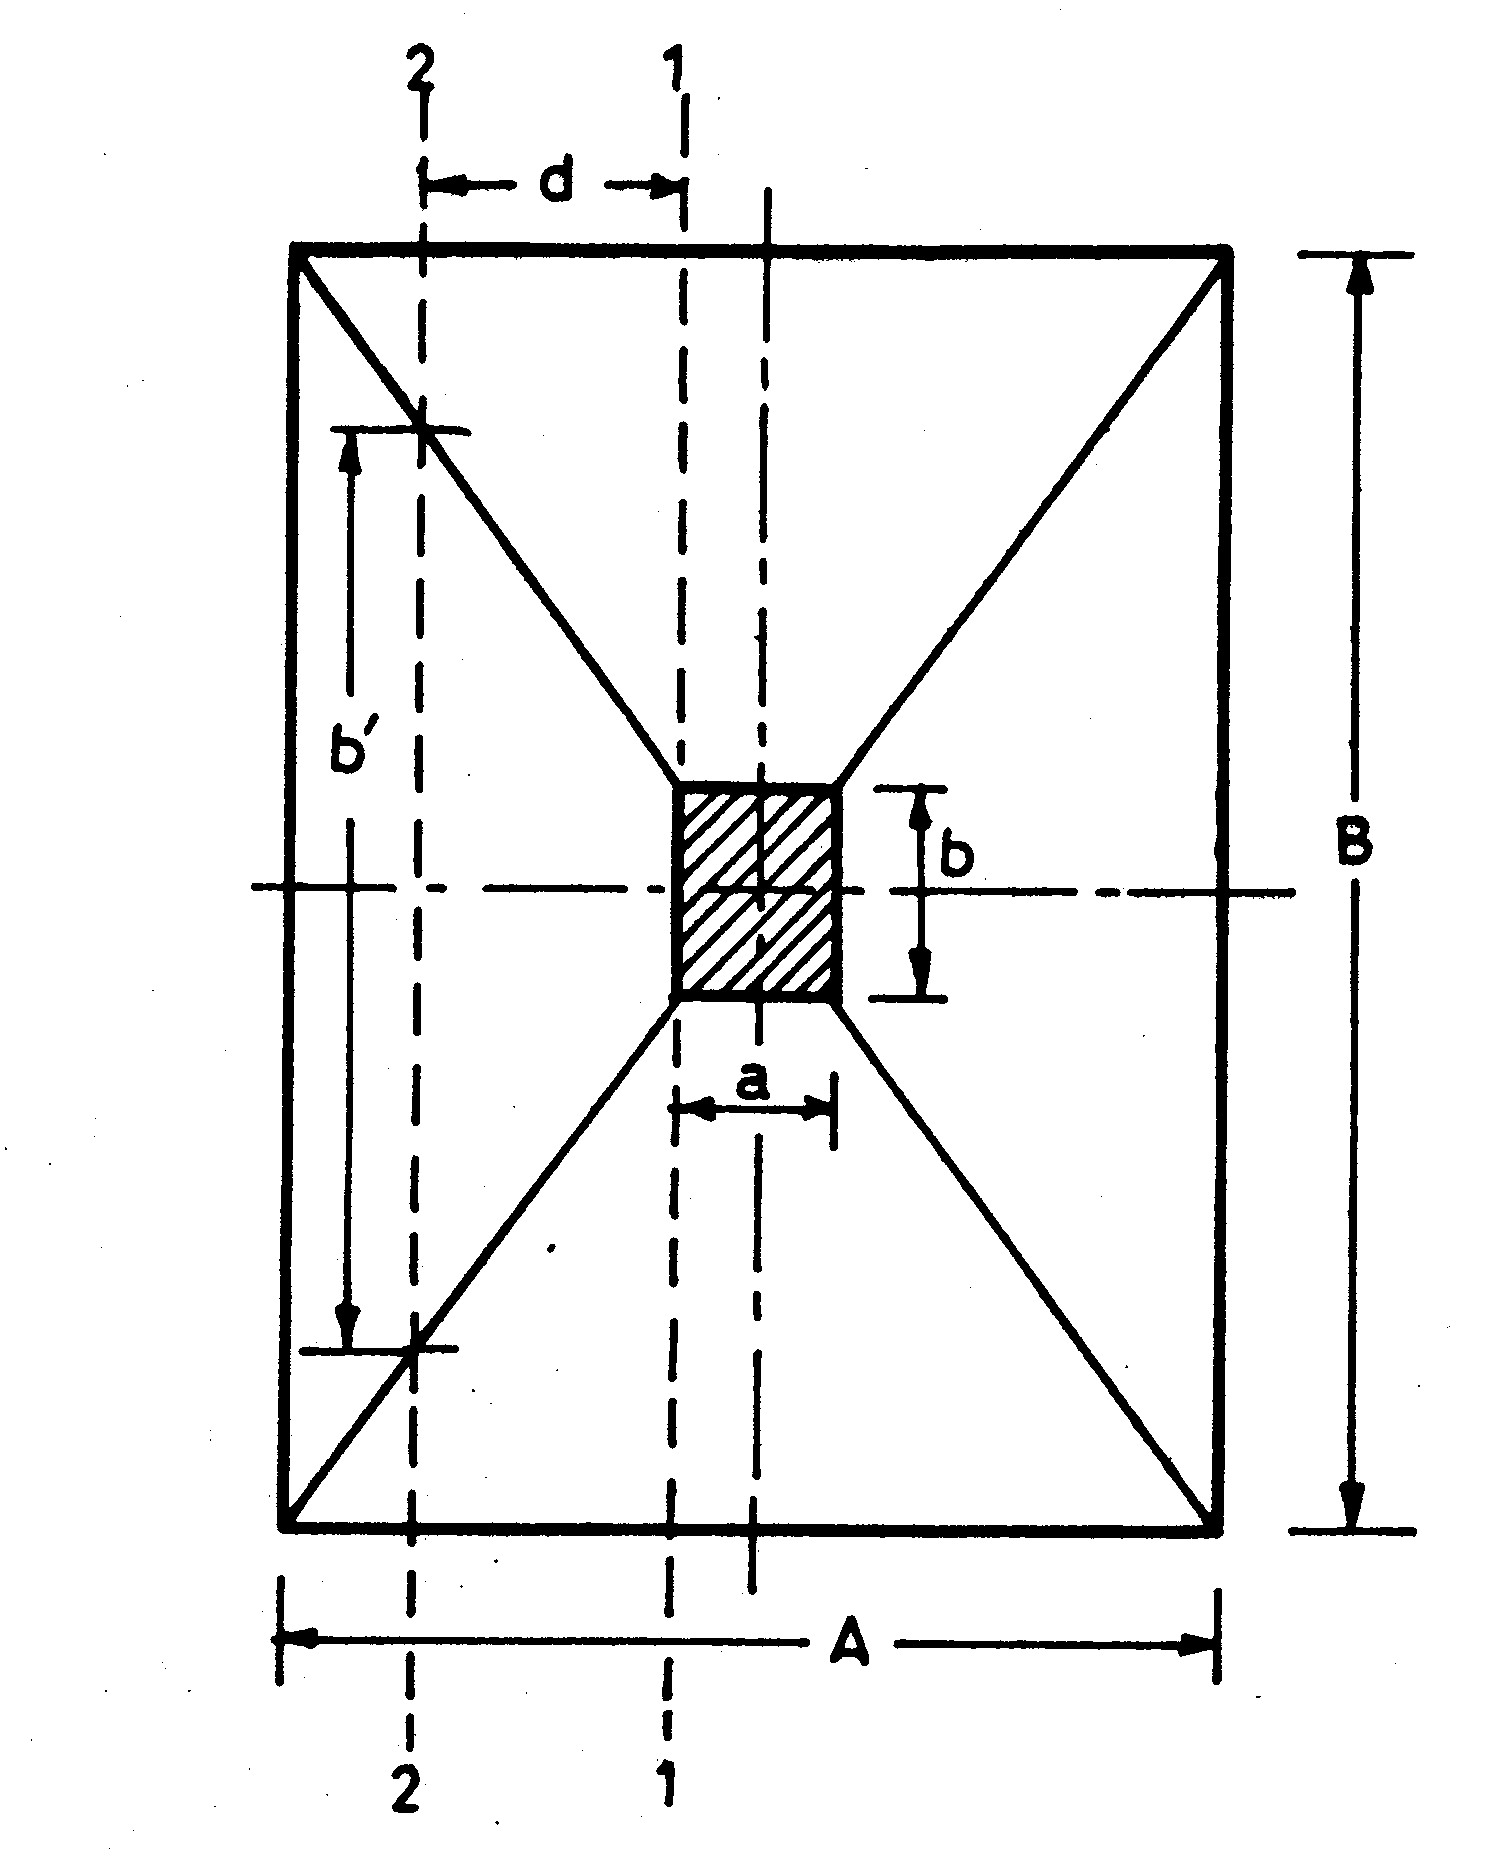
\includegraphics[width=\textwidth]{images/fig2321.png}
    \caption{Plan of sloped footing}
    \label{Planofslopedfooting}
  \end{subfigure}\\
  %
  \begin{subfigure}[b]{0.5\textwidth}
    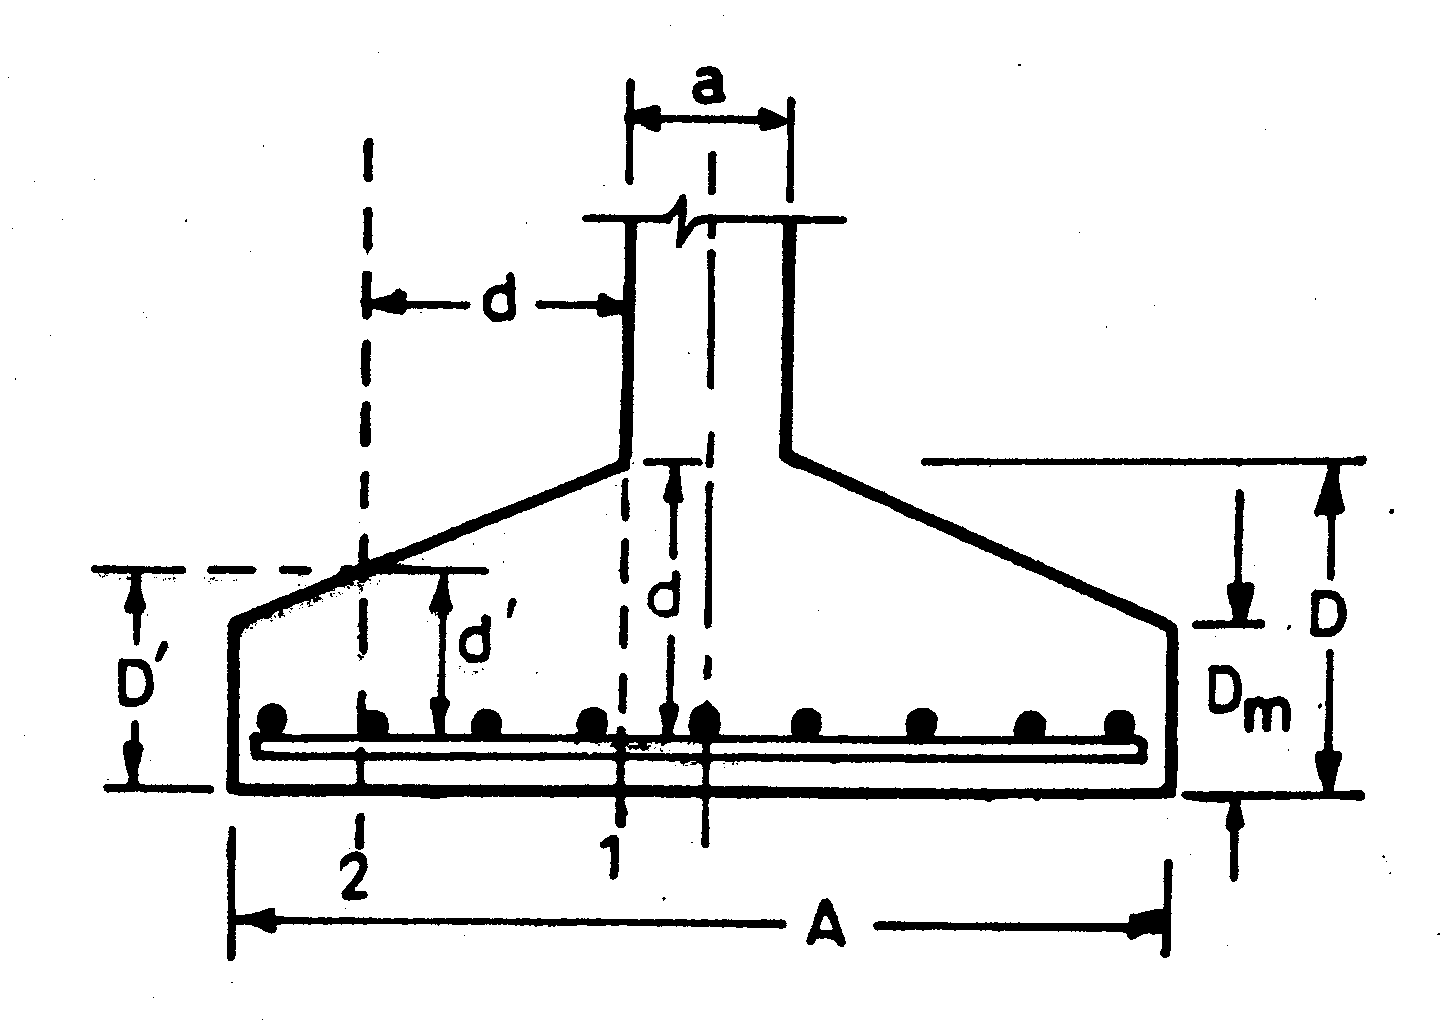
\includegraphics[width=\textwidth]{images/fig2322.png}
    \caption{Section of sloped footing}
    \label{sectionofslopedfooting}
  \end{subfigure}
\caption{Critical sections for bending moment and beam shear in footings.}
\label{critical-sections-for-bending-moment-and-beam-shear-in-footing}
\end{figure}%--------------------end figure-------------------%
Beam shear stress $\sage{tau_v}$ for footings of uniform depth and stepped footings is given by,

\begin{equation}
         \label{eq:shearstress22}
        \sage{tau_v}=\sage{z}= \frac{{1.5} \times S_{2-2}}{bd}
\end{equation}
where, $$b = \text{B for uniformaly deep footings,}$$ 
$$= \text{a for stepped footing} (\figmacro \ref{steppedfooting})$$
For sloped footings, clause 40.1.1 of the  \citetitle{IS2000} gives, (-ve sign applies here),

\begin{equation}
         \label{eq:clause40.1.1}
        \sage{tau_v}=\frac{\quad{V_u}}{b'd'}-\frac{M_u}{b'd'^2}.tan\beta
\end{equation}
where b', d' are shown in \figmacro \ref{Planofslopedfooting} and \figmacro \ref{sectionofslopedfooting} and ${M_u}$ is the ultimate moment at section 2-2.

\begin{sagesilent}
        var('D_m,D,a,A,d')
        z=D_m+((D-D_m)*(1-(a/A)-2*(d/A))/(1-(a/A)))
        var('phi,c')
        z2=c+phi
        var('b,B')
        z3=b+2*((B-b)/(A-a))*d
        be=var('beta')
        z4=tan(be)
        z5=2*((D-D_m)/(A-a))
        z6=2*(D-D_m)/(A-a-D)
\end{sagesilent}
\begin{equation}
        \label{eq:ultimatemoment22}
        D'=\sage{z}
\end{equation}

\begin{equation}
         \label{eq:ultimatemoment22b}
        d'=D'-(\sage{z2})
\end{equation}

\begin{equation}
         \label{eq:ultimatemoment22c}
        b'=\sage{z3} \sage{be}
\end{equation}

For Type (c), \figmacro \ref{slopefooting} gives,
\begin{equation}
         \label{eq:12.19}
        \sage{z4}=\sage{z5}
\end{equation}


For Type (b), \figmacro \ref{Slopedfooting} gives,
\begin{equation}
         \label{eq:12.20}
        \sage{z4}=\sage{z6}
\end{equation}

\begin{sagesilent}
        var('k,tau_a,tau_v,tau_c')
        z=k*tau_c
        var('V_v')
        z2=V_v/(b*d)
\end{sagesilent}
The calculated value of $\sage{tau_v}$ must not exceed the allowable stress $\sage{tau_a}$, as shear reinforcement is just not provided in individual footings for reasons of economy, the same as in solid slabs. The allowable stress in concrete solid slabs $\sage{tau_a}$ is given by,

\begin{equation}
         \label{eq:concretesolidslabs}
        \sage{tau_a}=\sage{z}
\end{equation}
$\sage{tau_c}$ is given by \tablemacro 19 of the  \citetitle{IS2000} depending on the steel area provided for moment at the critical section 2-2 (the minimum value of $\sage{tau_c}$ is assumed for $p_t $$\leq$$ 0.15$ in \tablemacro 19 and

$$\begin{array}{l@{}l}
&{}k=1.0 \text{ for } D \geq 300 \text{mm}\\
&{}=1.1 \text{ for } D = 250 \text{mm}\\   
&{}=1.2 \text{ for } D = 200 \text{mm}\\
&{}=1.25 \text{ for } D = 175 \text{mm}\\   
&{}=1.30 \text{ for } D \leq 150 \text{mm}  
\end{array}$$
Normally, depth of footing given for perimeter shear (\chartmacro \ref{Dummy chart}) is more than adequate
to satisfy the requirements of beam shear. But when steel type  \Fefouronefivemacro and \Fefivezerozeromacro are used as reinforcement beam shear may govern the depth of footing. For stepped footings, additional checks for moment and beam shear are required to be made for the portion of the footing of depth $D_m$ (\figmacro \ref{steppedfooting}). When section ${1'-1'}$ is the critical section for moment and section ${2'-2'}$ is that for beam shear (\figmacro \ref{steppedfooting}), expressions for moment and shear are given as,

\begin{equation}
         \label{eq:momentandshear1-1}
        M_{1'-1'}=p.B.\frac{(A-a')^2}{B}
\end{equation}

\begin{equation}                                             \label{eq:momentandshear2-2}
        S_{2'-2'}=p.B\bigg[\frac{(A-a')^2}{B}-d_m\bigg]                                 
\end{equation}
For finding steel area, \chartmacro 4.1 (with $\gamma = 0$), may be used, as the concrete compression zone is of a rectangular shape of width equal to B. Shear stress $\tau_v$ is given by,

\begin{equation}
        \label{eq:Shearstress}
        \sage{tau_v}=\sage{z2}=\frac{1.5S_{2-2}}{B.d_m}
\end{equation}
and it must not exceed $\tau_a$ given by \equmacro (\ref{eq:concretesolidslabs}), failing which depth $D_m$ should be suitably increased.
Normally $D_m = 0.30$ $D$ to $0.50$ $D$ is kept in stepped footings and perimeter shear stress can be checked to be safe by using first principles.

%------------------figure-------------------------------%
\begin{figure}
  \centering
  \begin{subfigure}[b]{0.5\textwidth}
    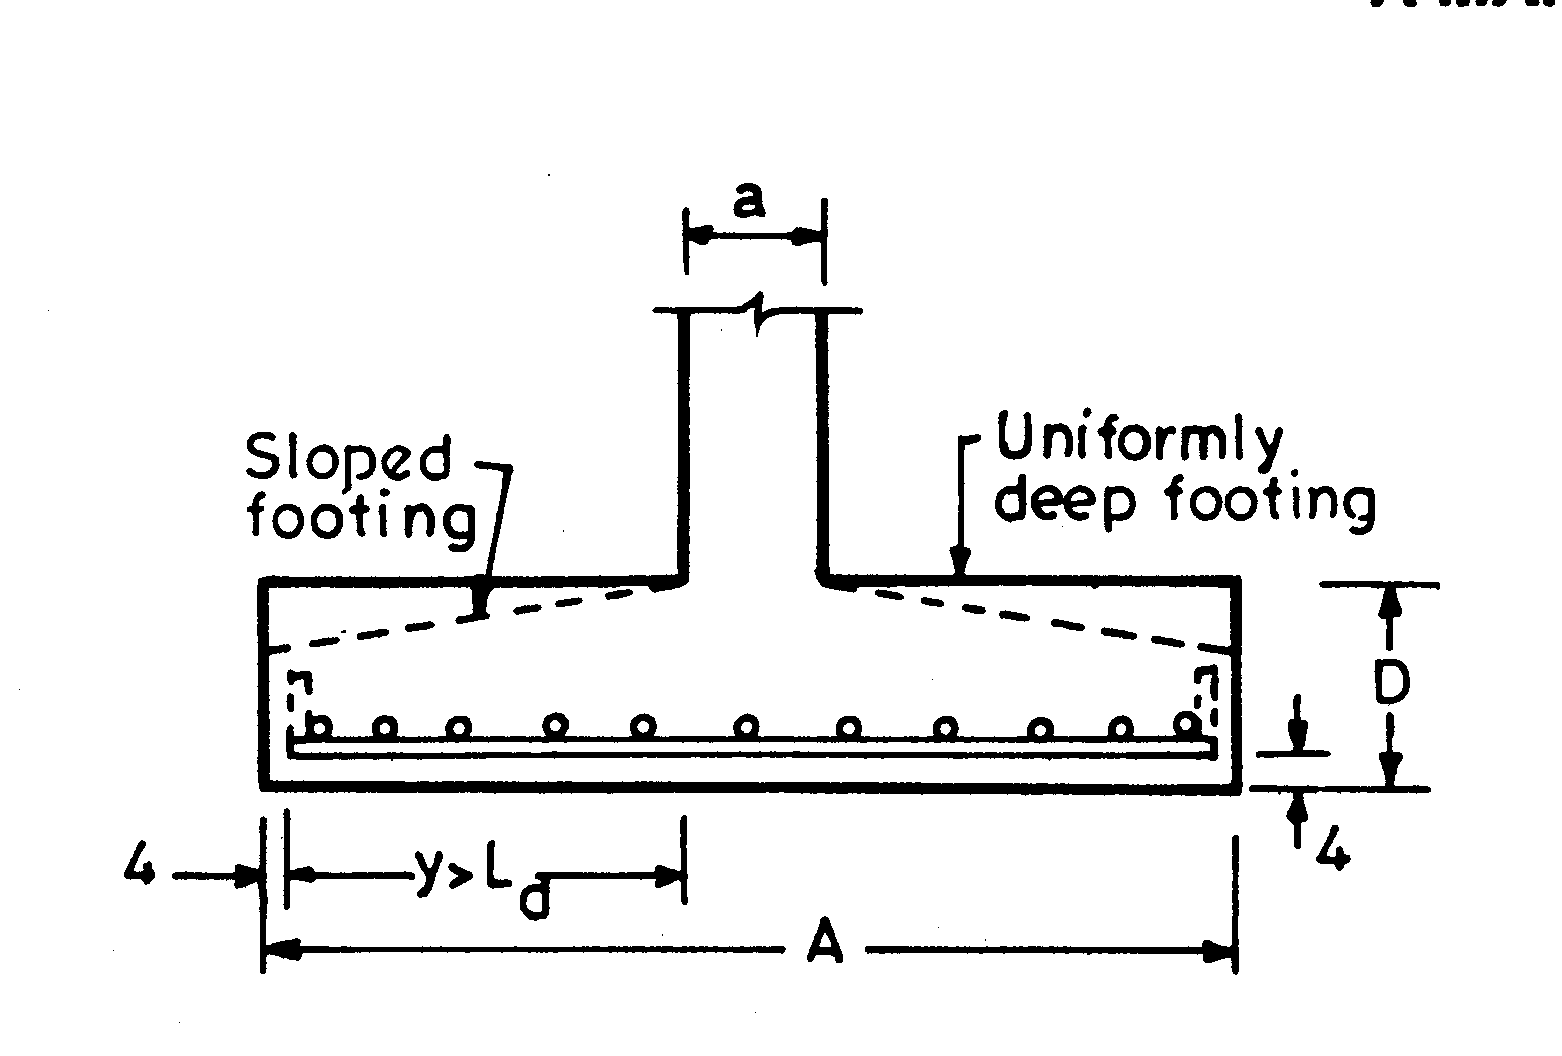
\includegraphics[width=\textwidth]{images/fig2341.png}
    \caption{Section of uniformaly and sloped footing}
    \label{uniformallydeepfooting}
  \end{subfigure}\\
  %
  \begin{subfigure}[b]{0.5\textwidth}
    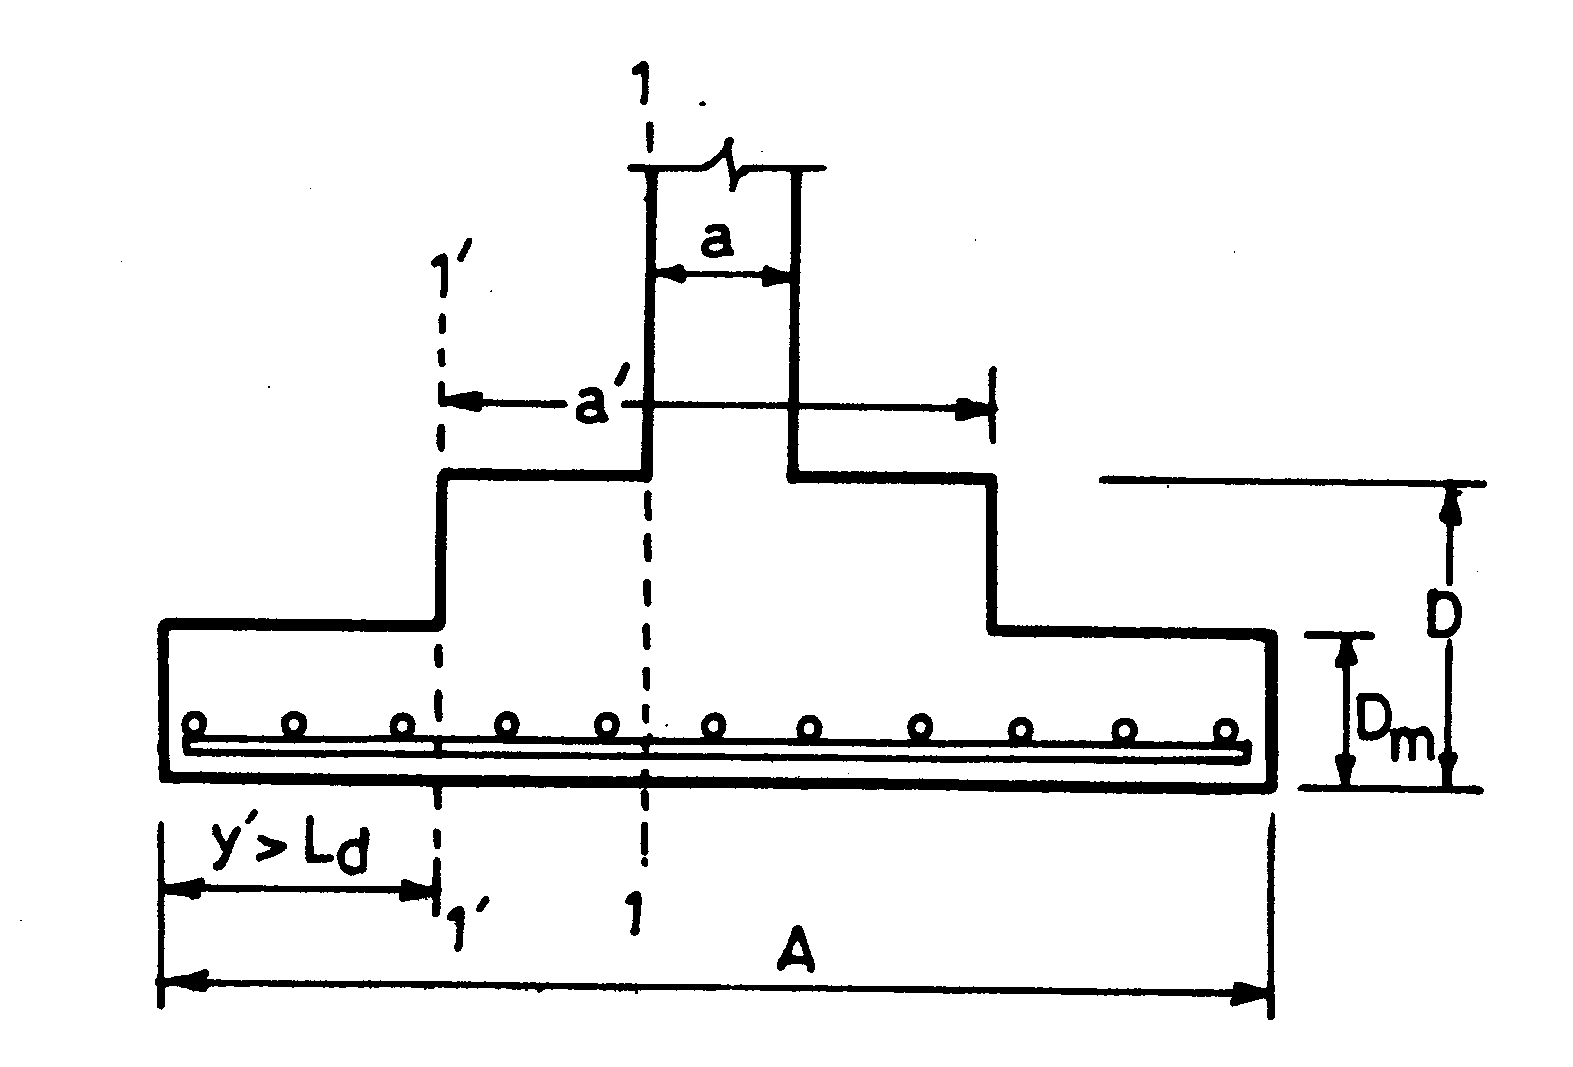
\includegraphics[width=\textwidth]{images/fig2342.png}
    \caption{Section of stepped footing}
    \label{stepedfoting}
  \end{subfigure}
\caption{Development length of footing bars.}
\end{figure}

%------------------end figure---------------------------%
\section{Development Length of Bars}
Column dowel bars should extend into footings for a distance equal to the development
length (\tablemacro 11.3 of Chapter 11) of column bars in compression (or in tension when moment in column is large). With the clause 26.2.2.2 of the Code, column bars can always be adequately anchored in the footing, whatever be the depth of footing. 

\begin{sagesilent}
        z=((A-a)/2)-4                    
\end{sagesilent}

For development length of footing bars, there should be adequate bar length available $(y)$, either straight or bent-up or both measured from the face of column. Referring to \figmacro\ref{uniformallydeepfooting}, for sloped or uniformly deep footings,

\begin{equation} 
        \label{eq:uniformallydeepfooting}
        y= \sage{z} >L_d (tension)
\end{equation}
where 40 $mm$ is taken as clear cover over ends of bars in footings. If \equmacro \ref{eq:uniformallydeepfooting} is not  satisfied, there are two ways to tackle this problem :

\begin{enumerate}
\item bend bars up, as shown dotted in \figmacro \ref{uniformallydeepfooting}
\item choose smaller diameter for bars.
\end{enumerate}

For stepped footings \figmacro \ref{stepedfoting}, the available straight length of bars beyond the critical
section ${1' - 1'}$ is,
                                                          
\begin{equation}                                                           \label{eq:criticalsection1-1}
        y'= \frac{(A-a')}{2}-4 >L_d (tension)                                      
\end{equation}
Normally, full steel area required at section $1 — 1$ is provided throughout and the steel strength $\sigma_s$ at section 1’ - 1’ may be less than its maximum value of 0.87 $f_y$. The value of $L_d$ (tension) should be calculated for the appropriate value of $\sigma_s$.

\section{Selection of Type of Footings}
Footings of uniform depth (Type $a$), though commonly used in practice for reasons of ease in design and construction, are the costliest. These consume more concrete quantity (about 25\% to 45\%) than that by sloped footings. This type is suitable only for small footings with overall depth being restricted to, say, 30 cm.

For footings of intermediate size, sloped footings with slope starting from $\dfrac{D}{2}$ away from the edge of column
(Type $b$), are quite suitable. This type is quite economical giving concrete and steel quantities quite reasonable in comparison with other types. This type is easy to design as well as to execute. This type is recommended for most individual footings encountered in buildings with overall depth greater than 30 $cm$. The depth at the free end of footing may be kept at 15 $cm$, the specified minimum given by the Code. The depth ($D$) of this type of footing is kept the same as that for footings of uniform depth.

For large-sized footings, sloped footings with the slope starting from the edge of column
(Type $c$) or stepped footings (Type $d$) are preferred to other types, as these give the least quantities for concrete and steel consumption. The stepped footings give the least steel quantity, while the sloped footings (Type $c$), give the least concrete quantity. The depth for these types of footings works out to be about 20\% more than that for footings of uniform depth. Stepped footings are a little cumbersome in construction, while the sloped footings are easier in execution, albeit a little more labour-intensive than the footings of uniform depth.

%-----------------------------------first numerical example--------------------%

\section{Examples}
\textbf{ Example 12.1. Square footing of Uniform Depth (Type a).}\\
\textbf{ Given:}
$$P = 1000kN$$
$$p = .02 kN/cm^2$$
$$a = 40 cm$$
$$f_{ck} = 15 N/mm^2$$
$$f_y = 415 N/mm^2$$
\textbf{Solution:}
\begin{enumerate}
\item \textbf{Dimensions of footing}\\
        \equmacro \ref{eq:footingArea} gives,
        $$A^2=\frac{1000}{0.02}=50,000 cm^2$$
        $$A=223.6 cm$$
Provided $225 \times 225$ base and
        $$p = \frac{100}{225 \times 225} = 0.01975 kN/cm^2$$
        \tablemacro \ref{chaptertable} gives for p = 0.02, and steel \Fefouronefivemacro,
        $$\frac{D}{A} = \frac{1}{4.5} \text{ or } D = \frac{225}{4.5}=50 \text{cm}$$
\item   \textbf{Check for perimeter shear}
        \chartmacro \ref{Dummy chart} gives for,
        $$k=\frac{0.67\sqrt{15}\times 1.0}{0.01975}=13.14$$
        $$\frac{a}{A}=\frac{40}{225}=0.18$$
        $$\frac{d}{A} = 0.18$$
        $$d=0.18 \times 225 = 40.5$$
\equmacro \ref{eq:depth-cover} gives with $c = 4.0 cm,\phi=1.2cm$,   
        $$D=40.5+4.0+1.2=45.7 cm$$
        $$D = 50cm \text{ is safe.}$$
\item  \textbf{Design for moment}
\equmacro \ref{eq:criticalMoment} gives,
$$M_{1-1}=0.01975 \times225(225-40)^2/8=19011kN/cm$$
With rectangular compression zone, \chartmacro (2.2) gives for,
        $$d=50-4.0-1.2=44.8cm$$
        $$k=\frac{1.5\times19011}{1.5\times225\times(44.8)^2}=0.042$$
        $$\mu = 0.0475$$
        $$A_{st}=\frac{0.0475\times225\times44.8\times15}{0.87\times415}=19.89cm^2$$
        $$\frac{A_{st}}{A}=\frac{19.89}{2.25}=8.84cm^2/m $$
$\phi 12/12 c/c $ both ways provided giving an area$ = 9.42cm^2/m$

\tablemacro 11.4 gives the minimum tension steel area in footings taken as slab,
$$A_{st}(min)=0.12\times50=6.0cm^2/m$$
which is exceeded by that provided.
\item  \textbf{Design for beam shear}
        \equmacro \ref{eq:shear22} gives,
        $$S_{2-2}=0.01975\times225\bigg[\frac{225-40}{2}-44.8\bigg]=212kN$$
        \equmacro \ref{eq:shearstress22} gives
\begin{sagesilent}
       var('tau_v,tau_c,tau_a')
\end{sagesilent}
$$\sage{tau_v}=\frac{1.5\times212}{225\times44.8}=0.032kN/cm^2$$
For $$\frac{100A_{s}}{bd}=\frac{100\times9.42}{100\times44.8}=0.21,$$

Table 19 of the Code gives,
$$\sage{tau_c}=0.32N/mm^2$$
With
$$k = 1.0 $$
\equmacro \ref{eq:concretesolidslabs} gives, 
        $$\sage{tau_a}=\sage{tau_c}=0.032kN/cm^2$$
With        
$$\sage{tau_v}=\sage{tau_a}, D = 50 cm \text{ is safe}$$

\item  \textbf{Check on development length of footing bars}

\tablemacro (11.13) gives, for footings bars of $\phi$ 12 (\Fefouronefivemacro),

$L_d$ (tension) = 55$\phi$ = 55 x 1.2 = 66 cm.

\equmacro \ref{eq:uniformallydeepfooting} gives, 

$$y=\bigg[\frac{(225-40)}{2}-4.0\bigg]=88.5cm$$

with $y > L_d$ (tension), footing bars will develop full strength at the critical section.

It may be noted that with $D$ = 50 $cm$, this type of footing of uniform depth is not economical. 
Footing of Types ($b$) and ($c$) with sloping depth would be more economical than the present design.
\end{enumerate} %--------second numerical example---------%
\textbf{ Example 12.2. Rectangular sloped footing of Type ($c$).}\\
\textbf{Given:}
Same as in Ex. 12.1 with
$$a = 40 cm$$
$$b = 60 cm$$ 
and the footing is to have equal overhangs on all sides of column.\\
\textbf{Required:} Design the footing\\
\textbf{Solution:}
\begin{enumerate}
\item   \textbf{Dimensions of footing}\\
  \equmacro \ref{eq:footingArea} gives,
  $$ A\times B= \frac{1000}{0.02}=50000 cm^2$$
  The equal overhang condition, \equmacro \ref{eq:shape} gives,
  $$ b-a=B-A=20 cm$$
  The solution of these two equations gives,
  $$A=214 cm$$
  $$B=234 cm$$
  Practical designer may choose A = 215 cm and B=235 cm
  $$p=\frac{1000}{215\times235}=0.0198  kN/cm^2$$
  \tablemacro \ref{chaptertable} gives for $p$ = 0.02 and steel \Fefouronefivemacro,
 $$\frac{D}{A}=\frac{1}{4.5}\times1.20$$
 $$D=\frac{(215+23)}{2 \times 4.5} \times 1.20=60cm$$
 $$D=60 \text{cm and} D_m=15cm$$
 
\item  \textbf{Check for perimeter shear}\\
 \equmacro \ref{eq:depth-cover} gives, with c = 4.0 cm, $\phi$ = 1.2 cm,
 $$d=60-(4.0+1.2)=54.8cm$$
 \equmacro \ref{eq:shape} gives,
 $$ \alpha=\frac{15}{54.8}+\frac{(60-15)}{54.8}.\frac{\Bigg(1-\frac{40}{215}-\frac{54.8}{215}\Bigg)}{\Bigg(1-\frac{40}{215}\Bigg)}-\frac{(4.0+1.2)}{54.8}$$
 $$=\frac{1}{54.8}(15+30.91-5.2)=0.74$$
 \chartmacro \ref{Dummy chart} gives for,
 $$ k=\frac{0.067\sqrt{15}\times0.74}{0.0198}=9.70$$
 $$\frac{a}{A} \text{(average value)}=\frac{(43+60)/2}{(215+285)/2}=\frac{50}{225}=0.22$$
 $$\frac{d}{A}=0.195 \text{ or d}=0.195\times225=43.9 cm$$
 $$D=43.9+4.0+1.2=49.1 cm$$
 $$D=60 \text{cm is safe in perimeter shear.}$$
 
\item  \textbf{Design for moment}\\
   \equmacro \ref{eq:criticalMoment} gives,
   $$M_{1-1}=0.0198 \times 235(215-40)^2/8=17812 kN cm$$
   with trapezoidal compression zone, Chart 4.1 gives for,
   $$b=60cm, d=54.8 cm$$
   $$tan\beta =\frac{(D-D_m)}{(B-b)/2}=\frac{45}{87.5}=0.514$$
   $$\gamma=\frac{54.8}{60\times0.514}=1.8$$
   $$k=\frac{1.5 \times 17812}{1.5 \times 60 \times (54.8)^2}=0.099$$
   $$\mu=0.11$$
   $$A_{st}=\frac{0.11 \times 60 \times 54.8 \times 15}{0.87 \times 415}=15.03cm^2$$
   $$\frac{A_{st}}{B}=\frac{15.03}{2.25}=640 cm^2/m$$
  Minimum steel for average value of $D =\dfrac{(60+15)}{2}=37.5$ regarding footings as slabs,
  $$A_{st}(min)=0.12\times 37.5=4.20 cm^2/m$$
  Provide $\phi$ $12/17$ $c/c$ bothways, $area=6.65 cm^2/m$
  
\item  \textbf{Design for beam shear}
  \equmacro (\ref{eq:shear22})gives
  $$S_{2-2}=0.0198\times235\Bigg[\frac{(215-40)}{2}-54.8\Bigg]=152 kN$$
  \equmacro (\ref{eq:ultimatemoment22}) gives,
  $$D'=15+(60-15)\frac{\Bigg(1-\frac{40}{215}-2\times \frac{54.8}{215}\Bigg)}{\Bigg(1-\frac{40}{215}\Bigg)}$$
  $$=15+16.8=31.8 cm$$
  \equmacro (\ref{eq:ultimatemoment22b}) gives,
  $$ d'=31.8-5.2=26.6 cm$$
 \equmacro (\ref{eq:ultimatemoment22c}) gives,
  $$b'=b+2\frac{(B-b)}{(A-a)}\times d=65+2\times \frac{175}{175}\times 54.8=169.6 cm$$
  \equmacro (\ref{eq:moment22}) gives
  $$M_2-2=0.0198\times 235(87.6-54.8)^2/2=2488 kN cm$$ 
  \equmacro \ref{eq:clause40.1.1} gives,
  $$\tau_v=\frac{1.5\times 152}{169.6\times26.6}-\frac{1.5\times 2488}{169.6\times (26.6)^2}\times 0.514$$
  $$=0.050-0.016=0.034 kN cm^2$$
  For
  $$\frac{100A_s}{b'd'}\frac{100\times6.65}{100\times26.6}=0.25,$$
  \tablemacro 19 gives ${\tau_c}$ = 0.035 \text{$kN/cm^2$}
  $$k=1.0,  {\tau_a}= {\tau_c}=0.035 kN/cm^2>{\tau_u}=0.034 kN/cm^2,$$
$$D=60 \text{cm is safe in beam shear}$$  
  
\item  \textbf{Check on development length of footing bars}\\
\tablemacro (11.3)gives for $\phi$ 12 bars
$$L_d (tension)=55\times1.2=66cm$$
\chartmacro \ref{Dummy chart} Effective Depth (($d$) of Square Individual Footings for Safety in perimeter shear.
$$k=\frac{\Bigg[1-\left(\frac{a}{A}\right)^2
-2\left(\frac{a}{A}\right)^2\left( \frac{d}{A}\right)-\left(\frac{d}{A}\right)^2\Bigg]}{\Bigg[\left(\frac{a}{A}\right)\left(\frac{d}{A}\right)+\left(\frac{d}{A}\right)^2\Bigg]}$$
$$k=0.067\frac{\sqrt{f_{ck}}}{p}$$
\equmacro \ref{eq:uniformallydeepfooting} gives,
$$y=\Bigg[\frac{(215-40)}{2}-4.00\Bigg]=83.5 \text{cm } > 66 \text{cm OK,}$$
\end{enumerate}
%--------------sage graph--------------%
\begin{sagesilent}                                                      
        var('a,A,d,k')                                                  
        f(k)=(1-(a**2)-(2*(a**2)*(d))-(d**2))/((a*d)+d**2)              
        solve(f(k) == k,d)                                              
        f(d) = -1/2*(2*a^2 + a*k - sqrt(4*a^4 + a^2*k^2 - 4*a^2 + 4*(a^3 - a^2 + 1)*k + 4))/(k + 1)
        z1=plot(f(a=.05),k,0,100,ymin=0,ymax=.30,figsize=(6.5,3),color=("green"),   legend_label= "a/A = 0.05")
        z2=plot(f(a=.1),k,0,100,ymin=0,ymax=.30,figsize=(6.5,3),color=("red"),      legend_label= "a/A = 0.10")
        z3=plot(f(a=.15),k,0,100,ymin=0,ymax=.30,figsize=(6.5,3),color=("yellow"),  legend_label= "a/A = 0.15")
        z4=plot(f(a=.20),k,0,100,ymin=0,ymax=.30,figsize=(6.5,3),color=("blue"),    legend_label= "a/A = 0.20")
        z5=plot(f(a=.25),k,0,100,ymin=0,ymax=.30,figsize=(6.5,3),color=("brown"),   legend_label= "a/A = 0.25")
        z6=plot(f(a=.30),k,0,100,ymin=0,ymax=.30,figsize=(6.5,3),color=("orange"),  legend_label= "a/A = 0.30")
        zz=z1+z2+z3+z4+z5+z6                                            
                                                                      
\end{sagesilent}                                                        
\begin{chart}                                                             \begin{center}                                                     
        \sageplot{zz,axes_labels=   ['$k$','$d/A$']}                       
\end{center}                                                       \caption{Effective Depth $(d)$ of Square Individual Footings for Safety of perimeter shear}  
\label{Dummy chart}    
\end{chart}    

\textbf{Notes:}
\begin{enumerate}
\item  $fck$ in $N/mm^2$
\item $p$ in $kN/cm^2$b
\item For rectangular column $a\times b$
Assume $a=\dfrac{(a+b)}{2}$ as in approximation provided $a/b$ $\leq$ $0.50.$
\item Chart can be used for squarish rectangular footings provided an equal overhang is left beyond faces of column with $A=\dfrac{A+B}{2}$\\
For equal overhang $(b-a)=(B-A)$
\item $\alpha=1.0$ for types (a),(b) and (d)(\figmacro \ref{Types-of-individual-spread-footing})
\item $\alpha<1.0$ for type (c). Use \equmacro \ref{eq:shape}
\item $\alpha=\dfrac{D_m}{d}+\dfrac{D-D_m}{d}.\dfrac{\left(1-\dfrac{a}{A}-\dfrac{d}{A}\right)}{\left(1-\dfrac{a}{A}\right)}-\dfrac{(c+\phi)}{d}$
\end{enumerate}

\section{Conclusion}
Provisions of the Code on footings have been applied to individual spread footings, square, or rectangular in plan with depth uniform, varying or stepped. Design aids are given for  fixing depth of footings and checking it in respect of requirements of safety in perimeter shear.Procedure for design of footings for bending moment, shear and development length of tension steel bars is given in detail and examples are given to illustrate it. For a large-sized rectangular footing, a footing beam in the long direction will be more economical than the traditional isolated footing. Also, for large square footings, two cross footing beams with a uniform base slab will make for economy.

\begin{table}[h!]\centering
        \pgfplotstableset{% global config, for example in the preamble
            % these columns/<colname>/.style={<options>} things define a style
            % which applies to <colname> only.
            every head row/.style={before row=\toprule,after row=\midrule},
            every last row/.style={after row=\bottomrule}
            }
         \pgfplotstabletypeset[% local config, applies only for this table
            1000 sep={\,},
            columns/info/.style={
            fixed,fixed zerofill,precision=2,showpos,
            column type=r,
            }
            ]
            {chapter12.dat}
        \caption{Depth of Footing for Safe Bearing Capacity}
        \label{chaptertable}
\end{table}

\textbf{Note:}
\begin{enumerate}
\item \textbf{{'A'} is the average of sides of rectangular footing.
\item For sloped (type c) and stepped (type d) footings, increased depth given by
the above table by 20\%}.
\end{enumerate}
~\cite{is4562000}
~\cite{aci1981aci}
~\cite{aci31877}
\printbibliography
\end{document}
